\documentclass[ngerman,compress]{beamer}

\mode<presentation>
{
  \useoutertheme[footline=titleinstituteauthor]{c4}
  \useinnertheme{circles}
  \usecolortheme{c4}
  %\setbeamercovered{transparent}
  \setbeamercovered{highly dynamic}
}

\usepackage{babel}
\usepackage[utf8]{luainputenc}
\usepackage{fontspec}
\usepackage{listings}
\usepackage{color}
\usepackage{mathtools}

% Multimedia
%\usepackage{multimedia}

% sets the listings style
\definecolor{sh_comment}{rgb}{0.12, 0.38, 0.18 } %adjusted, in Eclipse: {0.25, 0.42, 0.30 } = #3F6A4D
\definecolor{sh_keyword}{rgb}{0.3, 0.3, 0.875}  % #5F1441
\definecolor{sh_string}{rgb}{0.875, 0.85, 0.11} % #101AF9

\lstset{basicstyle=\tiny\ttfamily,
	showspaces=false,
	showtabs=false,
	showstringspaces=false,
	columns=fullflexible,
	stringstyle=\color{sh_string},
	keywordstyle=\color{sh_keyword}\bfseries,
	commentstyle=\color{sh_comment}\itshape
	}

\title[STM32 - Schieberegister, SPI, I2C - u23 2013]
{\textbf{STM32 - Schieberegister, SPI, I2C}\\u23 2013}

\author[andy <andy@koeln.ccc.de>]
{andy, florob, gordin, ike, meise, tobix, zakx}

\institute[Chaos Computer Club Cologne]
{
Chaos Computer Club Cologne e.V.\\
http://koeln.ccc.de \\
}

\date{Cologne\\2013-10-28}

\pgfdeclareimage[height=1cm]{barcode}{./c4-logo}
\logo{\pgfuseimage{barcode}}


% Folgendes sollte gelC6scht werden, wenn man nicht am Anfang jedes
% Unterabschnitts die Gliederung nochmal sehen möchte.
%\AtBeginSection[]
%{
%  \begin{frame}<beamer>
%    \frametitle{Gliederung}
%    \tableofcontents[currentsection,currentsubsection]
%  \end{frame}
%}

% Falls Aufzählungen immer schrittweise gezeigt werden sollen, kann
% folgendes Kommando benutzt werden:
%\beamerdefaultoverlayspecification{<+->}


\begin{document}

\begin{frame}
  \titlepage
\end{frame}

\AtBeginSubsection

\begin{frame}
  \tableofcontents
  % Die Option [pausesections] könnte nützlich sein.
\end{frame}



\section{Schieberegister}


\subsection{Schieberegister}

\begin{frame}
	\frametitle{Was ist das?}
	\begin{itemize}
		\item Register: Hält Daten
		\item Schieben: Die Daten werden hinein``geschoben''
		\item Vorteil: Viele Inputs/Outputs mit wenigen µC-Pins
		\item Nachteil: Höherer Programmieraufwand / Zeit- / Rechenbedarf
	\end{itemize}
\end{frame}

\begin{frame} [fragile]
	\frametitle{Funktionsweise}
	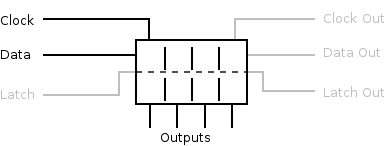
\includegraphics[width=2in]{01_funktionsweise.png}
\end{frame}

\begin{frame} [fragile]
	\frametitle{Funktionsweise}
	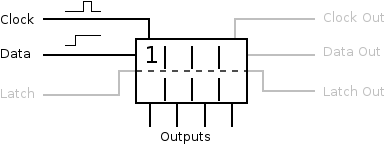
\includegraphics[width=2in]{02_shift.png}
	\pause
	\begin{itemize}
		\item Data: Eingehende Daten
		\item Clock: Bei steigender Flanke wird der Wert von Data in das temporäre Register übernommen
	\end{itemize}
\end{frame}

\begin{frame} [fragile]
	\frametitle{Funktionsweise}
	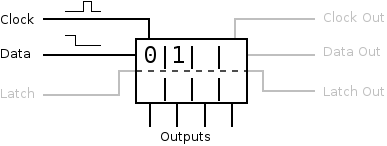
\includegraphics[width=2in]{03_shift.png}
	\pause
	\begin{itemize}
		\item Die Werte werden immer in das erste Feld übernommen
		\item Die vorhandenen Werte werden ``durchgeschoben''
	\end{itemize}
\end{frame}

\begin{frame} [fragile]
	\frametitle{Funktionsweise}
	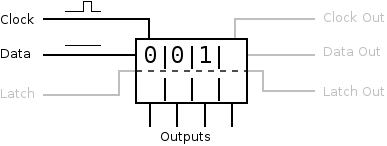
\includegraphics[width=2in]{04_shift.png}
	\begin{itemize}
		\item Die Werte werden immer in das erste Feld übernommen
		\item Die vorhandenen Werte werden ``durchgeschoben''
	\end{itemize}
\end{frame}

\begin{frame} [fragile]
	\frametitle{Funktionsweise}
	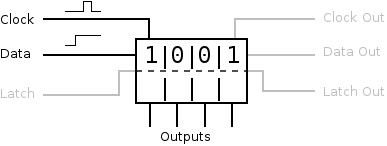
\includegraphics[width=2in]{05_shift.png}
	\begin{itemize}
		\item Die Werte werden immer in das erste Feld übernommen
		\item Die vorhandenen Werte werden ``durchgeschoben''
	\end{itemize}
\end{frame}

\begin{frame} [fragile]
	\frametitle{Funktionsweise}
	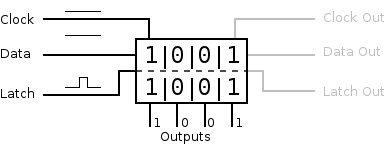
\includegraphics[width=2in]{06_latch.png}
	\pause
	\begin{itemize}
		\item Latch: Bei steigender Flanke werden die Werte des temporären Registers in das
			Output-Register übernommen
		\item Sonst werden diese Werte nie geändert!
	\end{itemize}
\end{frame}

\begin{frame} [fragile]
	\frametitle{Funktionsweise}
	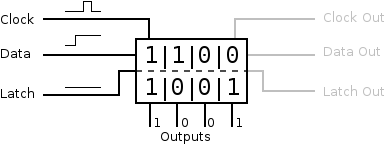
\includegraphics[width=2in]{07_shift.png}
	\begin{itemize}
		\item Latch: Bei steigender Flanke werden die Werte des temporären Registers in das
			Output-Register übernommen
		\item Sonst werden diese Werte nie geändert!
	\end{itemize}
\end{frame}


\subsection{Codebeispiel}

\begin{frame} [fragile]
	\frametitle{Bitbanging}
	\begin{itemize}
		\item Wie generiert man so ein Signal?
		\item Eine Möglichkeit: Manuelles Erzeugen mit GPIO's (``Bitbanging'')
		\item Jedes Bit wird einzeln generiert
	\end{itemize}
\end{frame}

\begin{frame} [fragile]
	\frametitle{Bitbanging Shiftbrites - Output}
	\begin{lstlisting} [language=C]
// Write a single 32 bit integer out to SPI by bitbanging.
// Also toggles the corresponding LED pins.
void gpiospi_write_int32(uint32_t data)
{
  // Go through the bits, MSB first
  for (int i=31; i>=0; i--)
  {
    // Get current bit
    uint32_t bit = data & (0x1<<i);

    // Set Data
    GPIO_WriteBit(GPIOB, GPIO_Pin_15, bit ? SET : RESET); // Data
    GPIO_WriteBit(GPIOD, GPIO_Pin_15, bit ? SET : RESET); // LED
    wait_own(wait_data);

    // Set clock high
    GPIO_WriteBit(GPIOB, GPIO_Pin_13, SET); // Clock
    GPIO_WriteBit(GPIOD, GPIO_Pin_13, SET); // LED
    wait_own(wait_data);

    // Set clock low
    GPIO_WriteBit(GPIOB, GPIO_Pin_13, RESET); // Clock
    GPIO_WriteBit(GPIOD, GPIO_Pin_13, RESET); // LED
    wait_own(wait_data);
  }
}
	\end{lstlisting}
\end{frame}

\begin{frame} [fragile]
	\frametitle{Bitbanging Shiftbrites - Latch}
	\begin{lstlisting} [language=C]
// Sets the latch pin (PIN 12) to high and then to low.
// At the same time also toggle the corresponding LED pins.
void latch(void)
{
  // Latch High
  GPIO_WriteBit(GPIOB, GPIO_Pin_12, SET); // Latch
  GPIO_WriteBit(GPIOD, GPIO_Pin_12, SET); // LED
  wait_own(wait_latch);

  // Latch Low
  GPIO_WriteBit(GPIOB, GPIO_Pin_12, RESET); // Latch
  GPIO_WriteBit(GPIOD, GPIO_Pin_12, RESET); // LED
  wait_own(wait_latch);
}
	\end{lstlisting}
\end{frame}

\begin{frame} [fragile]
	\frametitle{Bitbanging Shiftbrites}
	\begin{itemize}
		\item Der Code ist synchron
		\item Das heißt, die CPU ist die ganze Zeit damit beschäftigt die Daten rauszupusten
		\item Das dauert lange und kostet Rechenzeit
		\item Bitbanging ist die einfachste, aber nicht die Beste Lösung
		\item (siehe später)
	\end{itemize}
\end{frame}

\begin{frame} [fragile]
	\frametitle{Logic Analyzer}
	%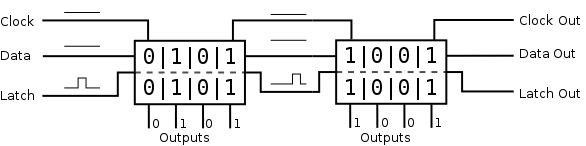
\includegraphics[width=4in]{15_latch.png}
	%TODO
	TODO
\end{frame}


\subsection{Chaining}

\begin{frame} [fragile]
	\frametitle{Jetzt wird's lustig}
	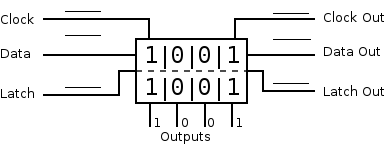
\includegraphics[width=2in]{08_outs.png}
	\pause
	\begin{itemize}
		\item Schieberegister haben noch mehr Funktionen:
		\begin{itemize}
			\item Data Out: Hier liegt der Wert des hintersten Datenbits an
			\item Clock Out: Das Clock Signal wird neu produziert / durchgeschleift
			\item Latch Out: Das Latch Signal wird neu produziert / durchgeschleift
		\end{itemize}
		\pause
		\item Data Out und Latch Out sind nicht immer vorhanden
	\end{itemize}
\end{frame}

\begin{frame} [fragile]
	\frametitle{Jetzt wird's lustig}
	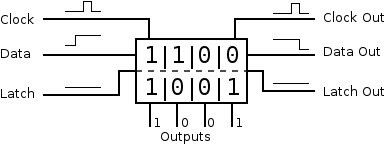
\includegraphics[width=2in]{09_shift.png}
	\begin{itemize}
		\item Schieberegister haben noch mehr Funktionen:
		\begin{itemize}
			\item Data Out: Hier liegt der Wert des hintersten Datenbits an
			\item Clock Out: Das Clock Signal wird neu produziert / durchgeschleift
			\item Latch Out: Das Latch Signal wird neu produziert / durchgeschleift
		\end{itemize}
		\item Data Out und Latch Out sind nicht immer vorhanden
	\end{itemize}
\end{frame}

\begin{frame} [fragile]
	\frametitle{Chaining}
	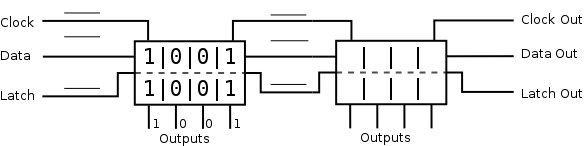
\includegraphics[width=4in]{10_chaining.png}
	\pause
	\begin{itemize}
		\item Man kann so mehrere Schieberegister hinter einander hängen
	\end{itemize}
\end{frame}

\begin{frame} [fragile]
	\frametitle{Chaining}
	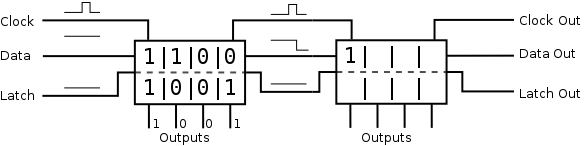
\includegraphics[width=4in]{11_chaining.png}
	\begin{itemize}
		\item Man kann so mehrere Schieberegister hinter einander hängen
	\end{itemize}
\end{frame}

\begin{frame} [fragile]
	\frametitle{Chaining}
	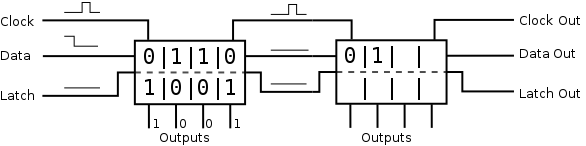
\includegraphics[width=4in]{12_chaining.png}
	\begin{itemize}
		\item Man kann so mehrere Schieberegister hinter einander hängen
	\end{itemize}
\end{frame}

\begin{frame} [fragile]
	\frametitle{Chaining}
	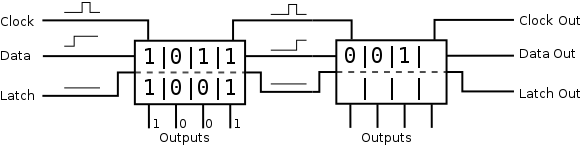
\includegraphics[width=4in]{13_chaining.png}
	\begin{itemize}
		\item Man kann so mehrere Schieberegister hinter einander hängen
	\end{itemize}
\end{frame}

\begin{frame} [fragile]
	\frametitle{Chaining}
	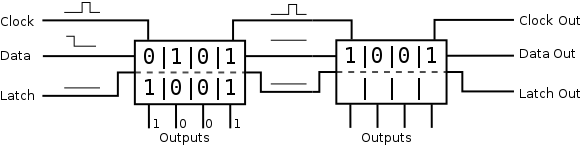
\includegraphics[width=4in]{14_chaining.png}
	\begin{itemize}
		\item Man kann so mehrere Schieberegister hinter einander hängen
	\end{itemize}
\end{frame}

\begin{frame} [fragile]
	\frametitle{Chaining}
	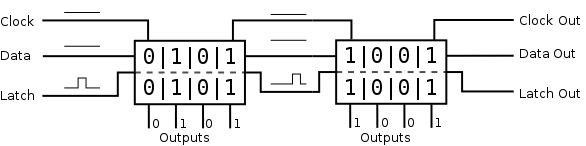
\includegraphics[width=4in]{15_latch.png}
	\begin{itemize}
		\item Man kann so mehrere Schieberegister hinter einander hängen
	\end{itemize}
\end{frame}



\section{SPI}


\subsection{SPI}

\begin{frame} [fragile]
	\frametitle{Was ist das?}
	\begin{itemize}
		\item SPI = \textbf{S}erial \textbf{P}eripheral \textbf{I}nterface
		\item Ein low-level Datenübertragunsprotokoll
		\item Seriell: Daten(bits) werden seriell (nacheinander) übertragen
	\end{itemize}
\end{frame}

\begin{frame} [fragile]
	\frametitle{Protokoll}
	\begin{itemize}
		\item Ähnlich zu Schieberegistern, allerdings:
		\item Es gibt keinen Latch, die Übertragung ist nach fester Bitlänge abgeschlossen
		\item Der Master gibt dem Slave ein Signal, dass dieser Slave angesprochen wird
			und die Übertragung beginnt. (sog. Chip Select)
		\item Es gibt einen Rückkanal
		\item Es wird immer gleichzeitig empfangen und gesendet
		\item Will man nur lesen, sendet man zB 0x00
	\end{itemize}
\end{frame}

\begin{frame} [fragile]
	\frametitle{Pins}
	\begin{itemize}
		\item CLK: Clock
		\item MOSI: Master Out Slave In
		\item MISO: Master In Slave Out
		\item CS: Chip Select
	\end{itemize}
\end{frame}

%\begin{frame} [fragile]
%	\frametitle{Logic Analyzer}
%	%\includegraphics[width=4in]{...}
%	%TODO Hab ich nicht gemacht
%\end{frame}


\subsection{Codebeispiel}

\begin{frame} [fragile]
	\frametitle{Initialisierung - Pins}
	\begin{lstlisting} [language=C]
// SPI  (SCK PB13, MISO PB14, MOSI PB15)
GPIO_Init(GPIOB, &(GPIO_InitTypeDef){
    .GPIO_Pin = GPIO_Pin_13 | GPIO_Pin_14 | GPIO_Pin_15,
    .GPIO_Mode = GPIO_Mode_AF,
    .GPIO_Speed = GPIO_Speed_50MHz,
  });

// Configure pins to be used by the SPI hardware (alternate function)
GPIO_PinAFConfig(GPIOB, GPIO_PinSource13, GPIO_AF_SPI2);
GPIO_PinAFConfig(GPIOB, GPIO_PinSource14, GPIO_AF_SPI2);
GPIO_PinAFConfig(GPIOB, GPIO_PinSource15, GPIO_AF_SPI2);
	\end{lstlisting}
\end{frame}

\begin{frame} [fragile]
	\frametitle{Initialisierung - SPI}
	\begin{lstlisting} [language=C]
// Init SPI
SPI_Init(SPI2, &(SPI_InitTypeDef){
    .SPI_BaudRatePrescaler = SPI_BaudRatePrescaler_64, // Configure Data speed
    .SPI_CPHA = SPI_CPHA_1Edge, // Sample data on rising edge
    .SPI_CPOL = SPI_CPOL_Low, // Clock is default low
    .SPI_CRCPolynomial = 1, // Don't use CRC
    .SPI_DataSize = SPI_DataSize_8b, // Send 8 bit at a time
    .SPI_Direction = SPI_Direction_2Lines_FullDuplex, // Enable Sending / Receiving
    .SPI_FirstBit = SPI_FirstBit_MSB, // Most Significant Bit first
    .SPI_Mode = SPI_Mode_Master, // STM32 is the master
    .SPI_NSS = SPI_NSS_Soft, // Don't use automatic chip select
  });

// Enable SPI hardware
SPI_Cmd(SPI2, ENABLE);
	\end{lstlisting}
\end{frame}

\begin{frame} [fragile]
	\frametitle{Initialisierung - Interrupts}
	\begin{lstlisting} [language=C]
// Enable SPI interrupt
NVIC_Init(&(NVIC_InitTypeDef){
    .NVIC_IRQChannel = SPI2_IRQn,
    .NVIC_IRQChannelPreemptionPriority = 0,
    .NVIC_IRQChannelSubPriority = 0,
    .NVIC_IRQChannelCmd = ENABLE,
  });
	\end{lstlisting}
\end{frame}

\begin{frame} [fragile]
	\frametitle{Daten Senden - Non-Buffered}
	\begin{lstlisting} [language=C]
// Enable RXNE interrupt
SPI_I2S_ITConfig(SPI2, SPI_I2S_IT_RXNE, ENABLE);

// Start Data transfer
SPI_I2S_SendData(SPI2, data);
	\end{lstlisting}
	\begin{itemize}
		\item Die SPI Hardware läuft nun Asynchron
		\item In der Zeit kann und wird die CPU etwas anderes tun (und wenn es nur warten ist)
		\item Zum Beispiel: Warten bis ein Byte komplett empfangen wurde
	\end{itemize}
	\begin{lstlisting} [language=C]
while (SPI_I2S_GetFlagStatus(SPI2, SPI_I2S_FLAG_RXNE) == SET);
	\end{lstlisting}
\end{frame}

\begin{frame} [fragile]
	\frametitle{Daten Senden - Interrupts}
	\begin{itemize}
		\item Besser mit Interrupts:
		\item Wenn die Übertragung vorbei ist und ein Byte empfangen wurde wird der RXNE
			(Receive Buffer Not Empty) interrupt ausgelöst
	\end{itemize}
	\begin{lstlisting} [language=C]
void SPI2_IRQHandler(void) {
  // Check for interrupt cause
  if(SPI_I2S_GetFlagStatus(SPI2, SPI_I2S_FLAG_RXNE) == SET)
  {
    data = SPI_I2S_ReceiveData(SPI2);
  }
}
	\end{lstlisting}
	\begin{itemize}
		\item Der Interrupt kann verschiedene Gründe haben, deswegen müssen wir prüfen ob es
			wirklich RXNE war
	\end{itemize}
\end{frame}

\begin{frame} [fragile]
	\frametitle{Daten Senden - Buffered}
	\begin{itemize}
		\item Wenn man mehr als ein Byte senden will, ist es übersichtlicher Buffer zu benutzen:
	\end{itemize}
	\begin{lstlisting} [language=C]
// Data structures
uint8_t buffer[3];
int RX_counter = 0;
int TX_counter = 0;

// Start transfer
SPI_I2S_ITConfig(SPI2, SPI_I2S_IT_RXNE, ENABLE);
SPI_I2S_ITConfig(SPI2, SPI_I2S_IT_TXE, ENABLE);
	\end{lstlisting}
	\begin{itemize}
		\item Wir benutzen einen weiteren SPI-Interrupt: TXE (Transmit Buffer Empty)
		\item Dieser wird aufgerufen sobald der interne Buffer der SPI leer ist
		\item In unserem Fall (SPI läuft nicht) passiert das sofort
	\end{itemize}
\end{frame}

\begin{frame} [fragile]
	\frametitle{Daten Senden - Interrupts}
	\begin{itemize}
		\item Wird TXE ausgelöst schreiben wir ein neues Byte
		\item Wenn wir alle geschrieben haben, deaktivieren wir TXE-Int
		\item Die gelesenen Bytes schreiben wir zurück in den Buffer (bei RXNE)
	\end{itemize}
	\begin{lstlisting} [language=C]
void SPI2_IRQHandler(void) {
  // Check for interrupt cause
  if(SPI_I2S_GetFlagStatus(SPI2, SPI_I2S_FLAG_RXNE) == SET)
  {
    buffer[RX_counter++] = SPI_I2S_ReceiveData(SPI2);
    if (RX_counter >= 3)
      SPI_I2S_ITConfig(SPI2, SPI_I2S_IT_RXNE, DISABLE);
  }

  else if(SPI_I2S_GetFlagStatus(SPI2, SPI_I2S_FLAG_TXE) == SET)
  {
    SPI_I2S_SendData(SPI2, buffer[TX_counter++]);
    if (TX_counter >= 3)
      SPI_I2S_ITConfig(SPI2, SPI_I2S_IT_TXE, DISABLE);
  }
}
	\end{lstlisting}
\end{frame}


\subsection{Schieberegister - die Zweite}

\begin{frame} [fragile]
	\frametitle{Schieberegister per SPI}
	\begin{itemize}
		\item SPI sieht fast so aus wie das Schieberegisterprotokoll
		\item Es fehlt nur der Latch
		\item Wir können Schieberegister also besser bedienen
		\item Der Latch muss allerdings ausgelöst werden, nachdem alle Daten geschrieben sind
		\item Wir müssen also warten bis die SPI fertig ist
		\item Dafür gibt es keinen Interrupt
		\item Man kann aber RXNE benutzen oder manuell warten
		\item Man sollte aber aufpassen mit dem Warten während eines Interrupts
	\end{itemize}
\end{frame}

\begin{frame} [fragile]
	\frametitle{Latch}
	\begin{lstlisting} [language=C]
void SPI2_IRQHandler(void) {
  // Check for interrupt cause
  if(SPI_I2S_GetFlagStatus(SPI2, SPI_I2S_FLAG_RXNE) == SET)
  {
    buffer[RX_counter++] = SPI_I2S_ReceiveData(SPI2);
    if (RX_counter >= 3)
    {
      while (SPI_I2S_GetFlagStatus(SPI2, SPI_I2S_FLAG_BSY) == SET);
      SPI_I2S_ITConfig(SPI2, SPI_I2S_IT_RXNE, DISABLE);
      latch();
    }
  }
  // [...]
}
	\end{lstlisting}
\end{frame}

\begin{frame} [fragile]
	\frametitle{Logic Analyzer}
	%\includegraphics[width=4in]{...}
	%TODO Hab ich nicht gemacht
\end{frame}

\begin{frame} [fragile]
	\frametitle{Ein Wort zu SPI Interrupts}
	\begin{itemize}
		\item TXE
		\begin{itemize}
		\item Wird ausgelöst wenn der Transmit Buffer leer ist
		\item Die SPI Hardware hat einen internen Buffer (8/16 bits)
		\item Und einen Schiebebuffer, aus dem die Daten herausgeschoben werden
		\item Das heißt die ersten beiden TXE-Ints kommen sehr schnell
		\item Und: Bei längerer Übertragung tritt der letzte TXE-Int beim vorletzten Byte auf
		\end{itemize}
		\item RXNE
		\begin{itemize}
		\item Tritt Nach jedem gelesenen Byte auf
		\item Liest man den RX-Buffer nicht aus, wird der Interrupt nochmal gefeuert!
		\item Wird der RXNE-Int blockiert (zB anderer Int), können Daten verloren gehen
		\end{itemize}
	\end{itemize}
\end{frame}

\begin{frame} [fragile]
	\frametitle{Logic Analyzer}
	%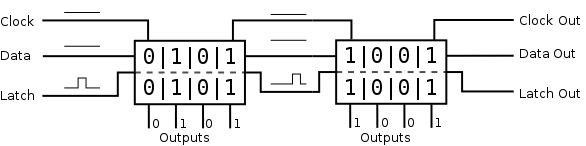
\includegraphics[width=4in]{15_latch.png}
	%TODO
	TODO
\end{frame}


\subsection{Bemerkungen}

\begin{frame} [fragile]
	\frametitle{SPI-Varianten}
	\begin{itemize}
		\item Es gibt viele Varianten von SPI
		\item Man kann vieles einstellen
		\item Siehe Datenblätter von Bauteilen
		\item und STM-Doku zur SPI-Initialisierung
	\end{itemize}
\end{frame}

\begin{frame} [fragile]
	\frametitle{SPI vs Shiftreg}
	\begin{itemize}
		\item Schieberegister brauchen nur 3 Pins, dafür Prozessorzeit
		\item SPI-Bausteine sind schneller zu bedienen, verbrauchen aber n+2 Pins
		\item Wahlweise kann man den Chip-Select mit Shiftregs bauen :) \\ $\rightarrow$ 5 Pins
	\end{itemize}
\end{frame}

\begin{frame} [fragile]
	\frametitle{Beispiele}
	\begin{itemize}
		\item Es gibt Beispiele
                \item libs/libsystem/\{inc,src\}/Spi.\{c,h\}
		\item bare\_metal/0*\_spi\_*
		\item Shiftbriteansteuerung per Bitbanging, SPI, und SPI+DMA
		\pause
		\item DMA ist ganz abgefahrenes Zeug, braucht ihr nicht
		\item Wenn doch / ihr Interesse habt / Masochisten seid: fragt uns
	\end{itemize}
\end{frame}
\end{document}
